\chapter{Poisson Brackets, Generators, and Angular Momentum}

We return here to Poisson brackets in the same spirit as the lecture itself: not as a fresh formalism dropped from the sky, but as the combination that keeps reappearing whenever we differentiate phase-space functions along motion. These companion notes follow Leonard Susskind's Lecture 8 closely; in this edition the chapter-production workflow is credited to LazyingArt LLC and Video2Book, while the mathematical development is taken from the lecture itself. The path is deliberate: first a recap, then a test on the harmonic oscillator, and only after that the real payoff, namely angular momentum, symmetry, generators, and finally the gyroscope.

\section{From Hamilton's Equations to the Poisson Bracket}

We begin with an arbitrary smooth function \(f(p,q)\) on phase space. If the system moves, the phase-space point \((q_i,p_i)\) moves, and therefore \(f\) changes along the trajectory. The first question is simply: what is \(\dot f\)?

By the chain rule,
\begin{equation}
\dot f=\sum_i \frac{\partial f}{\partial q_i}\dot q_i+\sum_i \frac{\partial f}{\partial p_i}\dot p_i.
\end{equation}
Now we substitute Hamilton's equations,
\begin{equation}
\dot q_i=\frac{\partial H}{\partial p_i},\qquad \dot p_i=-\frac{\partial H}{\partial q_i},
\end{equation}
and obtain
\begin{equation}
\dot f=\sum_i \frac{\partial f}{\partial q_i}\frac{\partial H}{\partial p_i}
-\sum_i \frac{\partial f}{\partial p_i}\frac{\partial H}{\partial q_i}.
\end{equation}

This combination occurs so often that it deserves a name of its own. For any two functions \(F(q,p)\) and \(G(q,p)\), we define the Poisson bracket
\begin{equation}
\{F,G\}=\sum_i \frac{\partial F}{\partial q_i}\frac{\partial G}{\partial p_i}
-\sum_i \frac{\partial F}{\partial p_i}\frac{\partial G}{\partial q_i}.
\end{equation}
With this notation, the previous formula becomes
\begin{equation}
\dot f=\{f,H\}.
\end{equation}

This is the point at which the lecture broadens its scope. The bracket is defined for any two functions \(F\) and \(G\), but only when the second entry is the Hamiltonian does it become a time derivative. That distinction matters later, because the same bracket will also describe rotations, translations, and other infinitesimal transformations.

\section{The Algebra of Poisson Brackets and the Harmonic Oscillator}

Once the bracket has been defined, we can treat it as an algebraic calculus. The basic rules are
\begin{align}
\{A,B\}&=-\{B,A\},\\
\{A+B,C\}&=\{A,C\}+\{B,C\},\\
\{\lambda A,B\}&=\lambda\{A,B\},\\
\{AB,C\}&=A\{B,C\}+\{A,C\}B.
\end{align}
Antisymmetry immediately gives
\begin{equation}
\{A,A\}=0.
\end{equation}
The canonical special cases are
\begin{equation}
\{q_i,q_j\}=0,\qquad \{p_i,p_j\}=0,\qquad \{q_i,p_j\}=\delta_{ij}.
\end{equation}

At this stage Susskind insists on doing a concrete calculation using only these rules, with no further appeal to Lagrange's equations and no re-derivation of Hamilton's equations. The chosen example is the harmonic oscillator,
\begin{equation}
H=\frac{p^2}{2m}+\frac{k}{2}q^2.
\end{equation}

We first compute \(\dot q\):
\begin{align}
\dot q
&=\{q,H\}\\
&=\left\{q,\frac{p^2}{2m}+\frac{k}{2}q^2\right\}\\
&=\frac{1}{2m}\{q,p^2\},
\end{align}
since \(q\) has zero Poisson bracket with any function of \(q\). Using the Leibniz rule,
\begin{align}
\{q,p^2\}&=\{q,pp\}=p\{q,p\}+\{q,p\}p=2p,
\end{align}
and therefore
\begin{equation}
\dot q=\frac{p}{m}.
\end{equation}

The second equation is equally direct:
\begin{align}
\dot p
&=\{p,H\}\\
&=\left\{p,\frac{p^2}{2m}+\frac{k}{2}q^2\right\}\\
&=\frac{k}{2}\{p,q^2\},
\end{align}
because \(p\) has zero bracket with any function of \(p\). Again by the Leibniz rule,
\begin{align}
\{p,q^2\}&=\{p,qq\}=q\{p,q\}+\{p,q\}q=-2q,
\end{align}
so that
\begin{equation}
\dot p=-kq.
\end{equation}
Combining the two,
\begin{equation}
m\ddot q=-kq.
\end{equation}

The oscillator proves that the machinery works. But it also sets up the lecture's next turn: so far the Poisson bracket has done little more than reproduce familiar equations in a new language. The real power appears when the distinguished quantity inside the bracket is not the Hamiltonian but a generator of symmetry.

\section{Angular Momentum From Rotational Symmetry}

The lecture now returns to the symmetry logic behind conserved quantities. Suppose we have an infinitesimal transformation
\begin{equation}
\delta q_i=F_i(q)\,\epsilon,
\end{equation}
with \(\epsilon\) a small parameter. The corresponding conserved quantity is
\begin{equation}
Q=\sum_i p_i F_i(q).
\end{equation}
As in the lecture, we suppress the overall factor of \(\epsilon\), since multiplying a conserved quantity by a fixed constant does not change the conservation statement.

For an infinitesimal rotation about the \(z\)-axis,
\begin{equation}
\delta x=-y\,\epsilon,\qquad \delta y=x\,\epsilon,\qquad \delta z=0.
\end{equation}
Substituting into the general symmetry formula gives
\begin{equation}
L_z=p_x(-y)+p_yx=xp_y-yp_x.
\end{equation}
This is the angular momentum for motion in the \(xy\)-plane, and in three dimensions it is naturally identified as the \(z\)-component.

Cycling the coordinates gives the remaining components:
\begin{equation}
L_x=yp_z-zp_y,\qquad
L_y=zp_x-xp_z,\qquad
L_z=xp_y-yp_x.
\end{equation}
Equivalently,
\begin{equation}
\mathbf L=\mathbf r\times \mathbf p.
\end{equation}
If we want the generator of rotation about some arbitrary axis \(\hat n\), we simply take
\begin{equation}
L_{\hat n}=\hat n\cdot \mathbf L.
\end{equation}

This is the point where the lecture stops treating angular momentum merely as a conserved quantity and starts asking what it does under Poisson bracketing.

\section{Angular Momentum as Generator of Rotations}

Before studying the Poisson brackets among the components of \(\mathbf L\), Susskind first brackets \(L_z\) with the coordinates themselves. This is presented explicitly as an exploration.

Using
\[
L_z=xp_y-yp_x,
\]
we find
\begin{align}
\{x,L_z\}&=-y,\\
\{y,L_z\}&=x,\\
\{z,L_z\}&=0.
\end{align}
The calculation is elementary but instructive. In \(\{x,L_z\}\), the only surviving contribution comes from the \(p_x\) term inside \(L_z\), and it produces \(-y\). Likewise, in \(\{y,L_z\}\), the only surviving contribution comes from the \(p_y\) term, and it produces \(x\).

The same pattern holds for the momentum components:
\begin{align}
\{p_x,L_z\}&=-p_y,\\
\{p_y,L_z\}&=p_x,\\
\{p_z,L_z\}&=0.
\end{align}
This is exactly the infinitesimal rotation law for the components of any vector. Position and momentum transform in the same way because both are vectors.

\subsection{Question \& Answer}

\paragraph{Question.} What does Poisson bracketing with angular momentum actually do?

\paragraph{Answer.} It gives the infinitesimal rotational change of whatever quantity we bracket with it. If \(A\) is any phase-space function, then the infinitesimal rotation about the \(z\)-axis generated by \(L_z\) is
\begin{equation}
\delta A=\epsilon\,\{A,L_z\}.
\end{equation}
The coordinate formulas above show this explicitly:
\[
\delta x=-y\,\epsilon,\qquad \delta y=x\,\epsilon,\qquad \delta z=0.
\]
So angular momentum is not only conserved because of rotational invariance; it also generates the rotation itself.

This is the same structural role that the Hamiltonian already played for time translations. In
\[
\dot A=\{A,H\},
\]
the Hamiltonian generates a small shift in time. Now we see that \(L_z\) generates a small rotation.

\section{Momentum, Translation, and the General Generator Idea}

The next step is to test the same idea on translations. For a small translation in a single coordinate \(q\),
\begin{equation}
\delta q=\epsilon.
\end{equation}
Here the symmetry function is simply \(F=1\), so the associated conserved quantity is the momentum \(p\). That already suggests the answer: momentum should generate translations.

Susskind then asks the key question in the lecture's own order. If \(f(q)\) is a function of \(q\), does Poisson bracketing with \(p\) give the small change in \(f\) under translation? In other words, does it give \(df/dq\)?

\subsection{Question \& Answer}

\paragraph{Question.} Does Poisson bracketing with momentum really give the infinitesimal translation?

\paragraph{Answer.} Yes, and the lecture proves it first for powers of \(q\), by induction.

\begin{proof}
For \(n=1\), the statement is just
\[
\{q,p\}=1,
\]
which is already in the canonical table.

Assume now that
\[
\{q^{n-1},p\}=(n-1)q^{n-2}.
\]
Then
\begin{align}
\{q^n,p\}
&=\{q\,q^{n-1},p\}\\
&=q\{q^{n-1},p\}+\{q,p\}q^{n-1}\\
&=q\bigl((n-1)q^{n-2}\bigr)+q^{n-1}\\
&=nq^{n-1}.
\end{align}
Thus the claim holds for \(n\), and since it holds for \(n=1\), it follows for all positive integers \(n\).
\end{proof}

So for powers of \(q\),
\begin{equation}
\{q^n,p\}=nq^{n-1}.
\end{equation}
By linearity, constant extraction, and the usual polynomial approximation argument, we recover the broader rule
\begin{equation}
\{f(q),p\}=\frac{df}{dq}
\end{equation}
for smooth \(f\).

Susskind jokes at this point that we need a verb for taking a Poisson bracket and proposes ``Poissonate.'' The joke is light, but the content is not. Poisson bracketing with momentum differentiates with respect to the translated coordinate. In the same sense in which \(L_z\) generates infinitesimal rotations and \(H\) generates infinitesimal time shifts, \(p\) generates infinitesimal translations.

\section{Conservation and Symmetry in One Equation}

By now the lecture has three distinguished examples in hand:
\begin{itemize}
\item the Hamiltonian generates time translations,
\item momentum generates spatial translations,
\item angular momentum generates rotations.
\end{itemize}
Susskind now gives them a common name: generators. Let \(G\) be any generator. Then the infinitesimal change of a quantity \(A\) under the \(G\)-generated transformation is
\begin{equation}
\delta_G A=\epsilon\,\{A,G\}.
\end{equation}

Now suppose \(G\) is conserved. Since time evolution is generated by \(H\), conservation means
\begin{equation}
\dot G=\{G,H\}=0.
\end{equation}
Using antisymmetry, we can read the same statement in the opposite order:
\begin{equation}
\{H,G\}=0.
\end{equation}
And now its meaning changes. The first equation says that \(G\) does not change in time. The second says that \(H\) does not change under the infinitesimal transformation generated by \(G\). That is precisely the symmetry statement.

\begin{figure}[h]
\centering

\includegraphics[width=0.66\textwidth]{lecture_08_figure_02.png}
\caption{The lecture isolates the two orders of the same vanishing Poisson bracket in order to emphasize their double reading: conservation of \(G\), and invariance of \(H\) under the transformation generated by \(G\).}
\end{figure}

The sparse board layout matters here. Susskind writes the two zero brackets one above the other, with a great deal of empty space around them, precisely to show that the same vanishing bracket can be read in two ways:
\begin{align}
\{G,H\}&=0,\\
\{H,G\}&=0.
\end{align}

\subsection{Question \& Answer}

\paragraph{Question.} If we know what is conserved, can we recover the symmetry?

\paragraph{Answer.} Yes. If we know a conserved quantity \(G\), then we bracket everything of interest with \(G\), and those brackets tell us how the variables transform:
\[
\delta_G A=\epsilon\,\{A,G\}.
\]
That does \emph{not} yet give the equations of motion. It gives the infinitesimal transformation generated by \(G\). Only when the generator is the Hamiltonian do these brackets become real time evolution.

This is one of the lecture's most important clarifications. The brackets with \(L_z\) tell us about rotational symmetry, not about particles moving in circles. The brackets with \(p\) tell us about translation symmetry, not about trajectories by themselves. Dynamics enters only when the generator is \(H\).

\section{Angular-Momentum Algebra and the Gyroscope}

The next step is to stop rebuilding angular momentum from coordinates every time and instead work directly with the Poisson algebra of its components.

A representative calculation is
\begin{align}
\{L_x,L_z\}
&=\{yp_z-zp_y,\;xp_y-yp_x\}\\
&=xp_z-zp_x\\
&=-(zp_x-xp_z)\\
&=-L_y.
\end{align}
That is exactly what one would expect for the \(x\)-component of a vector under a rotation generated by \(L_z\). Reordering and cycling the indices gives the standard angular-momentum algebra,
\begin{equation}
\{L_x,L_y\}=L_z,\qquad
\{L_y,L_z\}=L_x,\qquad
\{L_z,L_x\}=L_y.
\end{equation}

This is already a powerful simplification. We no longer need to return to the particle-by-particle definition of \(\mathbf L\) each time. The bracket structure itself can now be used as input.

\subsection{The Gyroscope}

The lecture closes with a gyroscope: a rapidly spinning wheel, attached at one point, with the distance from the pivot to the wheel center fixed. The important approximation is that the spin about the axle is so large that the dominant angular momentum remains aligned with the axle direction. In the lecture the notation shifts temporarily, but the clean reconstruction is
\begin{equation}
\mathbf L=\ell\,\mathbf r,
\end{equation}
where \(\mathbf r\) is the position vector from the pivot to the center of the wheel, and \(\ell\) is approximately constant because the spin is assumed very large. In particular,
\begin{equation}
L_z=\ell z.
\end{equation}

\begin{figure}[h]
\centering

\includegraphics[width=0.60\textwidth]{lecture_08_figure_03.png}
\caption{The first clear board appearance of the gyroscope geometry: a vertical \(z\)-axis, a pivot point, a slanted position direction, and the tilted flywheel.}
\end{figure}

\begin{figure}[h]
\centering
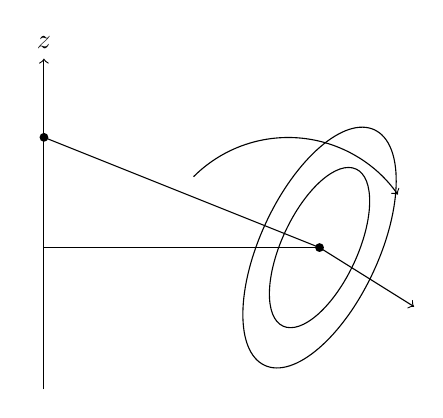
\begin{tikzpicture}[scale=1.0]
\draw[->] (0,0) -- (0,4.2) node[above] {$z$};
\fill (0,3.2) circle (1.6pt);
\coordinate (C) at (3.5,1.8);
\draw (0,3.2) -- (C);
\fill (C) circle (1.6pt);
\draw (0,3.2) -- (0,1.8);
\draw (0,1.8) -- (C);
\begin{scope}[shift={(C)}, rotate=-25]
\draw (0,0) ellipse (0.75 and 1.65);
\draw (0,0) ellipse (0.48 and 1.10);
\end{scope}
\draw[->] (1.9,2.7) arc[start angle=135,end angle=35,radius=1.7];
\draw[->] (C) -- +(1.2,-0.75);
\end{tikzpicture}
\caption{A clean redraw of the geometric picture used in the potential-energy argument. The vertical coordinate of the wheel center is \(z\), and the fast-spin approximation keeps \(\mathbf L\) aligned with the slanted position direction.}
\end{figure}

The rotational contribution to the Hamiltonian is
\begin{equation}
H_{\mathrm{rot}}=\frac{1}{2I}\left(L_x^2+L_y^2+L_z^2\right),
\end{equation}
with the corrected coefficient \(1/(2I)\). Susskind briefly says it incorrectly and then fixes it in the lecture; only the corrected form should be kept.

If there is no gravity, this is the whole Hamiltonian. Then, for example,
\begin{align}
\dot L_x
&=\{L_x,H_{\mathrm{rot}}\}\\
&=\frac{1}{2I}\Bigl(\{L_x,L_x^2\}+\{L_x,L_y^2\}+\{L_x,L_z^2\}\Bigr)\\
&=\frac{1}{2I}\Bigl(0+2L_y\{L_x,L_y\}+2L_z\{L_x,L_z\}\Bigr)\\
&=\frac{1}{I}\bigl(L_yL_z-L_zL_y\bigr)=0.
\end{align}
The same argument works for \(L_y\) and \(L_z\). Therefore, in the torque-free case,
\begin{equation}
\dot L_x=\dot L_y=\dot L_z=0.
\end{equation}
This is the familiar statement that without torque the angular momentum vector remains fixed.

\subsection{Question \& Answer}

\paragraph{Question.} Why is the gravitational potential proportional to \(L_z\)?

\paragraph{Answer.} Because in the fast-spin approximation the angular momentum vector stays aligned with the fixed-length position direction from the pivot to the wheel center. If we choose the vertical axis to be \(z\), and choose \(z\) to increase upward, then the gravitational potential is
\begin{equation}
V=Mg\,z.
\end{equation}
But \(L_z=\ell z\), so the same potential can be written as
\begin{equation}
V=cL_z,\qquad c=\frac{Mg}{\ell}>0.
\end{equation}
This is not an abstract identity; it uses the specific approximation that the spin angular momentum remains essentially along the axle direction.

\begin{remark}
A useful visual warning is that the cleaner board frame reproduced below still carries an earlier minus sign, \(V=-cL_z\). The lecture later corrects the sign in words. With the convention used here---\(z\) upward, so that larger height means larger potential energy---the cleaned formula is \(V=+cL_z\).
\end{remark}

\begin{figure}[h]
\centering

\includegraphics[width=0.72\textwidth]{lecture_08_figure_04.png}
\caption{The board later combines the gyroscope geometry with the rotational energy and an earlier-sign version of the potential term. The screenshot is kept as evidence of the live board layout; the cleaned formulas in the text follow the corrected sign convention.}
\end{figure}

Thus the full Hamiltonian, in the convention just fixed, is
\begin{equation}
H=\frac{1}{2I}\left(L_x^2+L_y^2+L_z^2\right)+cL_z.
\end{equation}
We already know that each \(L_i\) has zero Poisson bracket with \(L_x^2+L_y^2+L_z^2\), so only the \(cL_z\) term contributes to the evolution:
\begin{align}
\dot L_z&=\{L_z,H\}=c\{L_z,L_z\}=0,\\
\dot L_x&=\{L_x,H\}=c\{L_x,L_z\}=-cL_y,\\
\dot L_y&=\{L_y,H\}=c\{L_y,L_z\}=cL_x.
\end{align}
The vertical component remains fixed, while the horizontal components rotate into one another. This is the precession equation in the lecture's sense: the angular momentum vector sweeps around the \(z\)-axis instead of simply falling.

Susskind explicitly warns that he may have lost a sign by the end of the lecture. With the convention chosen here, these equations are the consistent cleaned form. The physical point, which the lecture emphasizes more than any sign bookkeeping, is that Poisson brackets let us write down the evolution directly for the angular-momentum components. We do not need to solve first for Euler angles and then reconstruct \(\mathbf L\); the useful variables come first.

The last analogy in the lecture is also worth keeping. Exactly the same bracket structure describes precession of spin in a magnetic field. The source of the torque may differ, but once a term linear in a component of angular momentum appears in the Hamiltonian, the algebra forces the same pattern of precession.

\section{Summary}

The lecture begins with a recap of \(\dot f=\{f,H\}\), but it does not stay there. The harmonic oscillator shows that Poisson brackets are operationally sound; angular momentum shows why they matter. Bracketing with \(L_z\) generates infinitesimal rotations, bracketing with \(p\) generates translations, and bracketing with \(H\) generates time evolution. The single condition \(\{G,H\}=0\) packages conservation and symmetry in one line, and the angular-momentum algebra then makes the gyroscope almost effortless. That is the lecture's central message: once the right bracket structure is in hand, mechanics can often be done directly in the variables that matter.